\documentclass[11pt]{article}
\usepackage[margin=0.7in]{geometry}
\usepackage{tikz,hyperref,booktabs}
\setlength{\parindent}{0pt}\setlength{\parskip}{7pt}
\begin{document}
\raggedright\sloppy
{\LARGE Pencil collector: first-gate observations}\\
Run \texttt{pencil-p739-20261030-a1}; snapshot 2026-10-30 00:30:41 UTC.

This report records observations from public synthetic known-answer mathematical workloads. It makes no mathematical or performance verdict. The original frozen protocol remains unchanged; reporting metadata corrections are explicitly post-data.

\textbf{Observed coverage.} All 60 prescribed targets are present in the fresh session: 1,080 execution records, including 180 warmups and 900 measured executions. The candidate/reference comparison has 300 prescribed measured pairs. All 1,080 records verified; native replay reproduced all 900 measured records with zero reported problems.

\begin{center}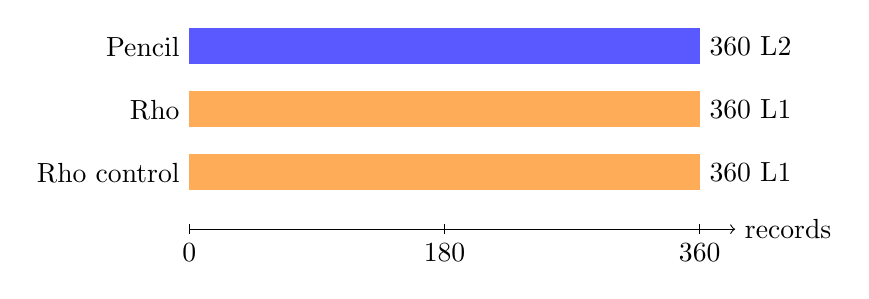
\begin{tikzpicture}[x=0.018cm,y=1cm]
\draw[->] (0,0)--(385,0) node[right]{records};
\foreach \v in {0,180,360}{\draw (\v,0.06)--(\v,-0.06) node[below]{\v};}
\fill[blue!65] (0,2.1) rectangle (360,2.55);
\fill[orange!65] (0,1.3) rectangle (360,1.75);
\fill[orange!65] (0,0.5) rectangle (360,0.95);
\node[left] at (0,2.32){Pencil};\node[right] at (360,2.32){360 L2};
\node[left] at (0,1.52){Rho};\node[right] at (360,1.52){360 L1};
\node[left] at (0,0.72){Rho control};\node[right] at (360,0.72){360 L1};
\end{tikzpicture}\end{center}
Each bar includes 300 measured executions and 60 warmups. Counts are observed totals, not estimates; no sampling uncertainty is assigned to these inventory counts. Source: \texttt{fresh-observed-counts.json} and the hash-bound raw records.

\textbf{Measurement acceptance.} Every pencil record reached L2; every rho and rho-control record was L1 because the solve interval was below the 1 ms L2 threshold. The fresh job exited 42 and the controller ended FAILED. Neither paired cold nor online timing is admitted. No qualified wall-time ratio is reported, and the measurement is not retried.

\textbf{Separate computation session.} The recovery computation also contains 1,080 verified records and 900 reproduced measured replays. Its clocks are explicitly invalid. It is retained separately and does not add another 60 distinct target identities to this gate.

\textbf{Price status at this snapshot.} The pinned native finite analyzer processed the full fresh gate. Its initial 36 cost cells are null pending the independent source/protocol/binary coverage binding. A later reviewed analysis can retain these observations without repeating solver work. The 1,260-target pencil objective remains incomplete; this gate covers 60 targets only.

\textbf{Resources and failures.} The earlier infrastructure attempt failed before payload spawn and retains a conservative 180-second reservation. That reservation is not measured worker time. The replacement controller ran from 00:15:44.603 to 00:26:26.317 UTC; the fresh worker container ran from 00:21:54 to 00:26:08 UTC. These are separate intervals and must not be summed as nonoverlapping mathematical work or converted to field operations. The original campaign deadline and budget were not extended.

\textbf{Review inputs.} This directory contains machine-readable JSON, CSV and SVG. Companion receipts are in \texttt{validation/actual\_gate\_results\_20261030/}; they bind raw records, versioned storage objects, native replay and analysis. Frozen v5 has four report-provenance metadata defects; the separate erratum preserves its original bytes and states that the correction followed data collection. No universal correctness theorem or external fastest-implementation comparison is established here.
\end{document}
